\chapter{Discussion \& perspectives}
\label{ch:discussion-perspectives}
{\hypersetup{linkcolor=GREYDARK}\minitoc}

As a legacy of the nearly-neutral theory, the evolution of molecular sequences is seen as a stochastic process.
One component of this process is creating diversity through mutation, while another antagonistic component is filtering out this diversity through selection, and finally the balance between these components is arbitrated by drift.
In the long term, this stochastic process results in a history of substitution events along species trees, inducing complex patterns of molecular divergence between species.
By analysing them, phylogenetic codon models aim at capturing the intrinsic parameters of evolution.

The focus of this thesis has been the development of new phylogenetic codon models and the modelling of the interplay between mutation, selection and drift in the evolutionary processes followed by protein-coding DNA sequences.
In this conclusive chapter, I first recall the main results of this thesis in section~\ref{sec:summary-of-main-results}.
Subsequently, I attempt to discuss the limitations of my work.
One main limitation concerns the problem of modelling site interdependence, which is discussed in section~\ref{sec:epistasis-and-entrenchment}.
Secondly, in section~\ref{sec:adaptative-landscape}, I draw some important connections between the mechanistic models developed here and the problem of detecting adaptive evolutionary regimes.
As a perspective, I discuss how phylogenetic mechanistic models could be unified with population genetics in section~\ref{sec:mechanistic-and-phenomenological-models}, and the inference methodology that would be adapted to such an endeavour in section~\ref{sec:mechanistic-and-phenomenological-models}.
Finally, before concluding, I discuss the question and the issue of reproducible sciences in evolutionary biology in section~\ref{sec:reproducible-science}.


\section{Summary of main results}
\label{sec:summary-of-main-results}

In chapter~\ref{chap:NucleotideBias}, I developed a phenomenological codon model in which $\omega$ is seen not as a single parameter but as a tensor (95 free parameters).
This sensor captures the small differences in fixation rate (or $\omega$) in different directions, which gives an accurate representation of how mutation and selection oppose each other at equilibrium.
This parameterization is the simplest one, in a phenomenological context, capable of correctly teasing apart mutation and selection.
Thanks to this, this modelling approach yields a reliable estimate of the mutational process, while disentangling fixation probabilities in different directions.

In chapter~\ref{chap:MutSelDrift}, I developed an extended mechanistic mutation-selection model reconstructing site-specific fitness landscape, long-term trends in effective population size and in the mutation rate along the phylogeny, from an alignment of \acrshort{DNA} coding sequences.
Simultaneously, the approach estimates the correlation between life-history traits, mutation rate and effective population size, intrinsically accounting for phylogenetic inertia.
Our framework was tested against simulated data and then applied to empirical data in mammals, isopods, primates and drosophila.
Simulated and empirical evidence suggest that there is a persistent signal in substitution patterns that relates to past history of $\Ne$, whose trends correspond to expected direction of correlation with life-history traits or ecological variables.
However, the magnitude of inferred variation in $\Ne$ across the phylogeny is narrower than expected, which is probably a bias of the approach caused by the assumptions made on the structure of the fitness landscape.

As a way to further investigate this last question, the third manuscript in chapter~\ref{chap:GenoPhenoFit} revisits the question of how the exact structure of the fitness landscape determines the quantitative response of the molecular evolutionary process, and in particular of $\dnds$, to changes in $\Ne$ and in protein expression level.
Specifically, I derive a theoretical approximation for the quantitative response of $\dnds$ to changes in both $\Ne$ and expression level, under an explicit genotype-phenotype-fitness map.
The development is generally valid for an additive trait under a log-concave fitness function, but was applied more specifically to a biophysical model in which proteins are under directional selection for maximizing their conformational stability.
In this specific case, I predict a weak response of $\dnds$ to changes in either $\Ne$ or expression level (which are interchangeable), a result corroborated by simulations under more complex models.
Based on this, I propose that fitness based on conformational stability might not provide a sufficient mechanism to explain the amplitude of the variation in the mean fixation probability which is observed empirically.
Other aspects of protein biophysics could be explored such as protein-protein interactions, which could lead to a stronger response of the mean fixation probability to changes in $\Ne$.

More globally, there is a remaining gap between quantitative predictions of biophysical models and empirical observations relating the response of protein coding sequence evolution to changes in $\Ne$ and expression level.


\section{Site interdependence and epistasis}
\label{sec:epistasis-and-entrenchment}

One of the blind spots of the mechanistic codon model developed in chapter~\ref{chap:MutSelDrift}, and more generally of current mechanistic models of the Halpern-Bruno family (see section~\ref{subsec:HB-formalism}), is the assumption of site independence.
This assumption is convenient, both computationally and statistically.
Computationally, each site can be considered as an independent Markov process (see sections~\ref{subsec:mutation-limited-assumption} and~\ref{sec-intro:likelihood}).
Statistically, one can rely on mixture models to estimate site-specific amino-acid fitness profiles (see section~\ref{subsec:empirical-calibration-HB})
In contrast, from a modelling and inference perspective, accounting for epistasis is challenging both in terms of parametrization and in terms of computational complexity (see section~\ref{subsec:structurally-constrained-site-interdependent-codon-models})
This complexity is the main reason why epistasis is generally ignored in phylogenetic models, and more particularly in codon models.
Empirically, however, evolutionary biologists have many reasons to believe that this hypothesis of site independence is not adequate, especially given our knowledge about protein biophysics (see section~\ref{subsec:conformational-stability-and-epistatis}).
This approximation is therefore problematic, and raises multiple questions.
What are the consequences of ignoring epistasis in the context of phylogenetic inference?
Practically, how could we ultimately account for epistasis in the context of inference?

Previous studies have argued that models of molecular evolution should consider the importance of epistasis for its different roles: from the importance in speciation, in modulating the rate of adaptation, in interlocking between sites (Stokes shift), downward impact on the $\dnds$ predicted by the mutation-selection models, and many other factors \citet{Goldstein2017, Miller2018}.
Based on our analysis presented in chapter~\ref{chap:GenoPhenoFit}, we argue that epistasis also has an important role in the response of $\dnds$ to changes in $\Ne$, both in terms of its susceptibility and dynamic of the response.
This is a conceptual point that, to your knowledge, had never been really identified until now.

More precisely, one key result of chapter~\ref{chap:GenoPhenoFit} is that any model without (or ignoring) epistasis implies a slow dynamic and a strong sensitivity of the mean fixation probability to changes in $\Ne$.
Intuitively, model without epistasis exhibit a slow return to equilibrium upon a change in $\Ne$ due to the waiting time until the next substitution.
Indeed, the evolutionary process is mainly mutation limited (see section~\ref{subsec:molecular-evolution-is-mutation-limited})
In addition, the mutation rate per site is very low, from $10^{-8}$ to $10^{-9}$ in mammals.
As a result, for each site, the expected waiting time until the next mutation is between $100$ to $1000$ million years, .
As for the strong sensitivity of the mean fixation probability to changes in $\Ne$, it originates in the fact that after a change in $\Ne$, each site of the sequence has to adapt independently, and change its position in the fitness landscape.

In contrast, in the presence of epistasis, the burden of adapting to changes in $\Ne$ is shared by more sites, such that not all of them (and possibly, very few of them) have to switch their position in the fitness landscape, in order for the trait to return to equilibrium under the new $\Ne$.
As a result, adding epistasis to the model implies a faster dynamic and a weaker response of the mean fixation probability to changes in $\Ne$.

These observations have several implications for empirical analyses.
First, if epistasis implies a weak response of the $\dnds$ to changes in $\Ne$, such as observed in chapter~\ref{chap:GenoPhenoFit}, for similar reasons, it may also explain the low magnitude of $\Ne$ variation estimated with site-specific mechanistic codon models in chapter~\ref{chap:MutSelDrift}.
Empirically, it appears that the susceptibility of $\dnds$ to changes in $\Ne$ is between these two extremes, namely that of site-specific fitness landscapes, and the other extreme of a single univariate phenotype controlled by all sites.
More probably, the ternary relation from sequence to phenotype to fitness implies several sites, but not all sites of the sequences, in a given phenotypic trait.

Second, the very long slow dynamic time constants implied by site-specific models are of the order of the depth of phylogeny ($100$ to $1000$ My).
As such, in the absence of epistasis, we shouldn't even see $\dnds$ correlations with either \acrshort{LHT} or $\Ne$ because of it.
Conversely, the fact that we see it is in itself an important indication of the presence of epistasis.

Ultimately, accounting for epistasis in mechanistic models of evolutions is necessary but challenging from a computational and statistical perspective.
Paths for statistical methods that can account for it are developed in section~\ref{sec:mechanistic-and-phenomenological-models}.

\section{Adaptive landscape and positive selection}
\label{sec:adaptative-landscape}

Another blind spot the mechanistic phylogenetic codon model developed in chapter~\ref{chap:MutSelDrift} is the absence of adaptive evolution (see section~\ref{subsec:where-is-adaptation?}).
Indeed, the mutation-selection equilibrium is essentially a nearly-neutral regime.
As a result, at mutation-selection equilibrium, the sequence is close to the fitness optimum and therefore, most mutations are deleterious or compensate for previous deleterious mutations that reached fixation.
Adaptation, on the other hand, can be seen as a process where the underlying fitness landscape is not fixed (i.e. time-independent) but is instead dynamic (i.e. time-dependent).
In other words, it is not so much a fitness landscape than fitness seascapes~\citep{Mustonen2009}.
Under a fitness seascape, the sequence is constantly running after a moving target, and as a result, there is net flux of adaptive substitutions (see section~\ref{subsec:adaptive-evolution}).

\subsection{Mechanistic mutation-selection models under fitness seascapes}
\label{subsec:mechanistic-fluctuating-selection}

In the context of a mutation-selection framework, explicitly modelling adaptation in terms of fitness seascapes fluctuating along the phylogeny appears to be challenging.
A first direction is to consider that adaptation consists in changes in the site-specific fitness profiles along some lineages.
These changes can either be informed by experimental mutational scanning~\citep{Bloom2017}, or estimated using a priori knowledge of phenotypic changes or ecological shifts\citep{Tamuri2009, Parto2018, Parto2018a}.
Without knowledge of the drivers of adaptation, modulations of the fitness profiles through time could also be implemented as a Markov modulated process along the phylogeny.
However, such an endeavour would be statistically and computationally challenging and might require to first rethink the entire statistical approach (see section~\ref{sec:mechanistic-and-phenomenological-models}).

\subsection{Hybrid mechanistic and phenomenological mutation-selection models}
\label{subsec:hybrid-mechanistic-and-phenomenological-mutation-selection-models}

As an alternative to explicit models of adaptation through fitness seascapes, the current nearly-neutral mutation-selection framework can be leveraged as a null model.
Deviation from this null model can be seen as a signal of adaptation (see section~\ref{subsec:adaptive-evolution}).
In particular, if the sequences are under recurrent positive selection, the mean fixation probability ($\avgpfix$) of non-synonymous mutations will tend to be higher than predicted by the purely nearly-neutral model.
This discrepancy between the mean fixation probability and the nearly-neutral expectation can be captured by a deviation parameter $\omega_*$, as in \citet{Rodrigue2016}.

Thus far, however, this idea has been implemented only at the gene level (i.e. invoking a single $\omega_*$ for the whole gene).
Yet, adaptation often occurs more locally, in specific domains of the protein.
Accordingly, this gene-wide deviation parameter $\omega_*$ could be refined at the site-level.
In this direction, in a work led by Nicolas Rodrigue, we developed a method to detect site-specific adaptation as a deviation from a null nearly-neutral model of evolution.
This method has been developed in the generic programming environment provided by \texttt{BayesCode} (see section~\ref{subsec:implementation}), and the manuscript accepted in the journal \textit{Molecular Biology \& Evolution} is available in appendix page~\pageref{sec-appendix:MutSelM3starMBE}.
These methods are relatively new, and must still be validated, more broadly applied to empirical data, and their predictions more extensively compared with those obtained from with classical codon models.

However, in its current form, phylogenetic model seeking adaptation as a deviation from near-neutrality assumes a constant $\Ne$ across the tree.
As already discussed, this assumption is of course not reasonable.
A simple solution to this problem would be to add a deviation parameter $\omega_*$ in the mechanistic model developed in chapter~\ref{chap:MutSelDrift}.
The resulting model would potentially be more effective at detecting positive selection.

Interestingly, $\omega_*$ could also be allowed to vary across branches, like $\Ne$.
This could have useful applications.
For instance, bats are known to be reservoirs of pathogens.
Recent results suggest they have more efficient immune system~\citep{Baker2013,Pavlovich2018}, such that proteins involved in host-pathogen interactions are under positive selection~\citep{Hawkins2019,Vandewege2020}.
But also, bats have large population sizes, compared to other mammals, and thus more efficient purifying selection.
These two factors have opposing effects on $\dnds$, and teasing them out might therefore be difficult using classical codon models.
In contrast, the mutation-selection model with both $\Ne$ and $\omega_*$ varying across lineages could offer a way to estimate them separately, which would allow to address the problems mentioned above.
Thus, do bats, compared to other mammals, have both stronger purifying selection (lower $\dnds$) due to large $\Ne$ and stronger positive selection (larger $\omega_*$)?

\subsection{Detecting adaptation with polymorphism}
\label{subsec:detecting-adaptation-with-polymorphism}

Phylogenetic codon models are only one of the methods currently available to detect adaptation.
There are other approaches that are widely used in population genetics, and that make use of the signal contained in polymorphism data, such as originally pioneered by \citet{McDonald1991}.
The idea behind the McDonald \& Kreitman (\acrshort{MK}) approach is to decompose the rate of selected substitutions ($\omega_{\text{Tot}}$), as a mixture of both advantageous substitutions and non-adaptive (nearly-neutral) substitutions:
\begin{align}
    \omega_{\text{Tot}} & = \omega_{\text{A}} + \omega_{\text{NA}}, \\
    \iff \omega_{\text{A}} & = \omega_{\text{Tot}} - \omega_{\text{NA}},
\end{align}
where $\omega_{\text{NA}}$ is the rate of substitution contributed by non-adaptive nearly-neutral evolution and $\omega_{\text{A}}$ is the total rate of substitution contributed by adaptive evolution.
In this context, under the assumption that adaptive mutations are rare, the ratio of non-synonymous over synonymous polymorphism ($\pnps$) mostly contains non-adaptive polymorphism and is a measure of $\omega_{\text{NA}}$:
\begin{equation}
    \omega_{\text{NA}} \simeq \pnps.
\end{equation}
Moreover, the total rate ratio of non-synonymous over synonymous substitutions ($\dnds$), estimated from divergence data, is a measure of $\omega_{\text{Tot}}$:
\begin{equation}
    \omega_{\text{Tot}} \simeq \dnds.
\end{equation}
Altogether, the rate of adaptive evolution, which contributes disproportionately to the divergence are estimated as the difference between divergence and polymorphism:
\begin{equation}
    \omega_{\text{A}} \simeq \dnds - \pnps.
\end{equation}

However, estimation of the non-adaptive rate through $\pnps$ can be biased by moderately deleterious mutations and by the change in population size through time~\citep{eyre-walker_changing_2002}.
To overcome these biases, a method initially proposed by \citet{eyre-walker_estimating_2009, Galtier2016} relies on the synonymous and non-synonymous site-frequency spectra (\acrshort{SFS}) to correct for demography and to estimate the distribution of fitness effects of mutations (\acrshort{DFE}), modelled as a continuous distribution.
This method, and subsequent developments which are reviewed in \citet{Moutinho2019a}, provide more reliable estimates of $\omega_{\text{NA}}$ and, as a result, a better estimate of $\omega_{\text{A}}$.

\subsection{Confronting methods for detecting adaptation}
\label{subsec:confronting-methods-for-detecting-adaptation}

The availability of independent phylogenetic methods (based on either phenomenological and mechanistic codon models) and population genetics approaches (using the McDonald \& Kreitman ideas) for detecting adaptation raises the question whether they detect congruent signals of adaptation.

Empirically, phenomenological and mechanistic codon methods should be confronted to McDonald \& Kreitman (\acrshort{MK}) methods.
In the case of the overlap between positively selected genes detected with phenomenological codon models and with \acrshort{MK} methods, the set of genes detected does not seem to overlap beyond random expectation~\citep{He2020}.
In contrast, at the site level, classical codon models are congruent with \acrshort{MK} methods, with most adaptive mutations occurring at the surface of proteins in both methods~\citep{Moutinho2019}.
These results still need be refined across clades and genes, and the availability of polymorphism and divergence \acrshort{DNA} sequences that are aligned will make this comparison possible.

However, positively selected genes or sites detected by classical codon models and \acrshort{MK} methods can theoretically be different, since non-adaptive part of substitution ($\omega_{\text{NA}}$) is subtracted in \acrshort{MK} test while classical codon models are not accounting for it.
Interestingly, another estimate of $\omega_{\text{NA}}$ in the context of phylogenetic codon model is what was referred to as $\omega_0$ in the context of the mutation-selection null model (see section~\ref{subsec:HB-formalism-nearly-neutral-model}).
As a result, mechanistic mutation-selection codon models ($\omega_0$) and \acrshort{MK} test ($\pnps$) should theoretically be more directly comparable.
From the availability of divergence and polymorphism data, it is now possible to ask whether the rate of non-adaptive evolution measured by phylogenetic mutation-selection models and \acrshort{MK} methods are congruent, and if not the reason for such discrepancy should be understood.

\begin{figure}[htbp]
    \centering
    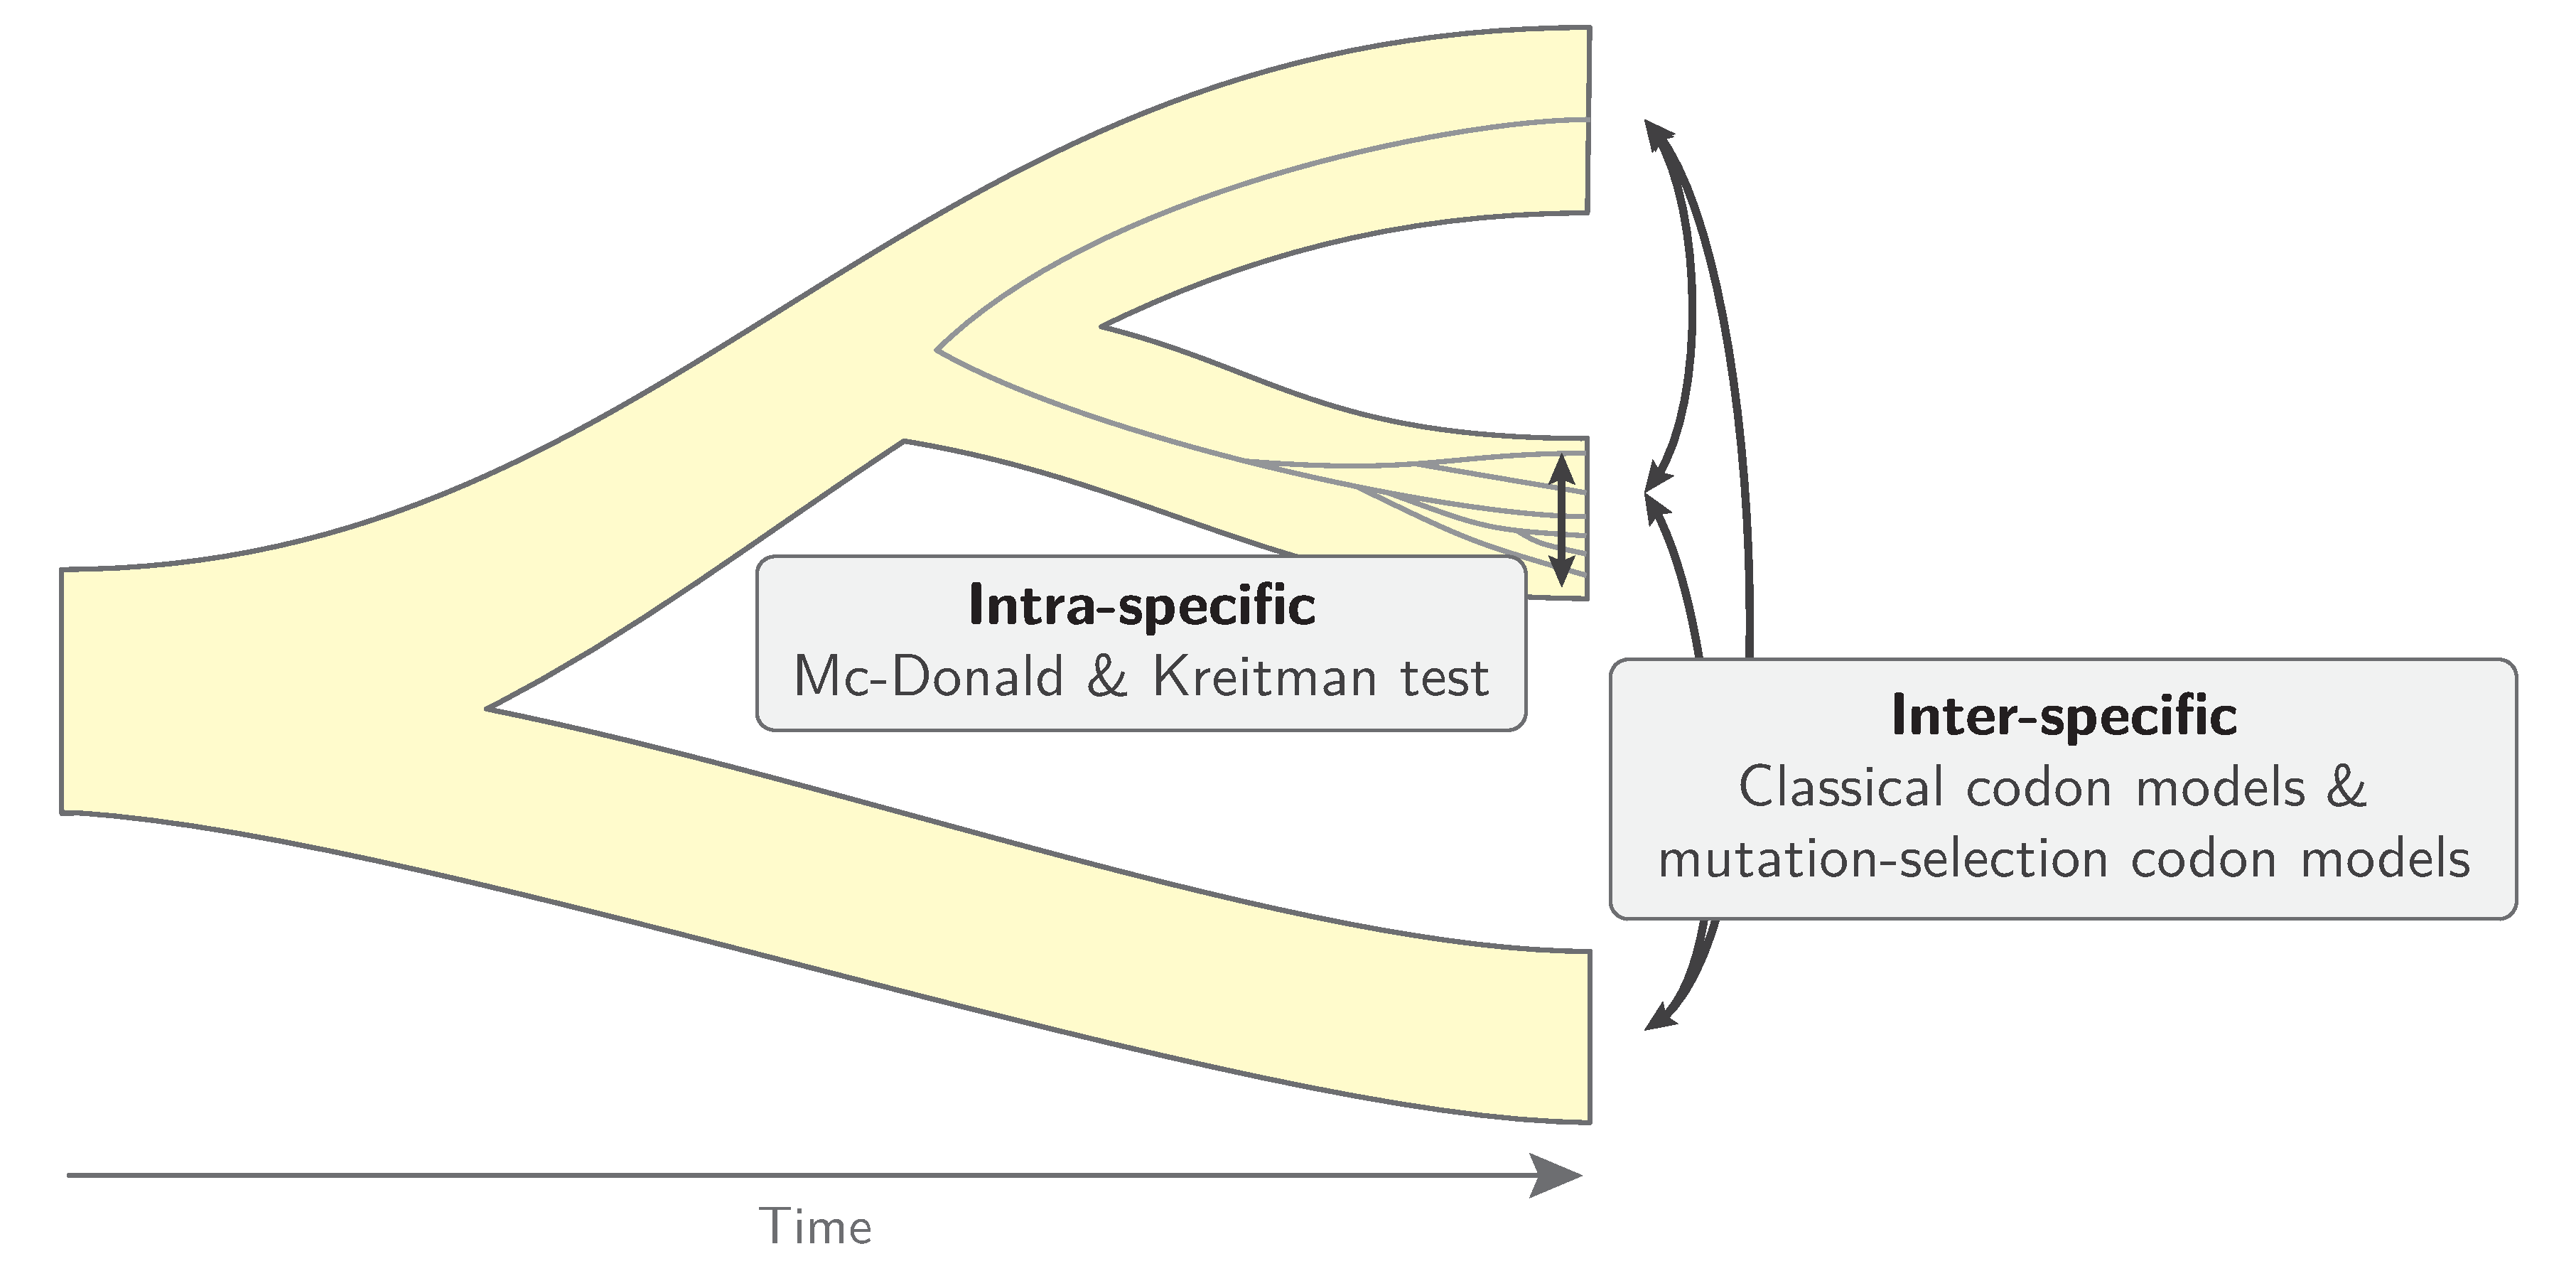
\includegraphics[width=\textwidth] {figures/inter-intra}
    \caption{Detecting adaptive evolution in coding sequences from inter- and intra-specific data}
    \label{fig:detecting-adaptation-inter-intra}
\end{figure}

\section{Unifying phylogenetic and population-genetics model}
\label{sec:unifying-phylogenetic-and-population-genetics-model}

Throughout this manuscript, the phylogenetic codon models that have been presented have so far ignored genetic diversity within species.
As a result, all differences observed in the alignment are assumed to be substitutions.
However some of the differences observed in the alignment might in fact be polymorphisms segregating in the population.
Moreover, substitutions are not instantaneous and ancestral shared polymorphisms can result in incomplete lineage sorting~\citep{Charlesworth2010}.

Mistaking polymorphisms for substitutions is problematic, since both are not sensitive to mutation, selection and drift to the same extent~\citep{Mugal2014}.
For example, the neutral diversity increases with $\Ne$, while the rate of neutral substitutions is insensitive to $\Ne$.
Also, mildly deleterious can be present in polymorphism while being filtered out by selection and not present in substitutions.

Finally, substitution rates are much more strongly influenced by selection, and more generally by fixation biases (such as gBGC) than polymorphisms, which are primarily reflecting mutation biases.

Interestingly, this suggests that polymorphism and divergence could be leveraged together to help disentangle mutation, selection and drift.
In other words, phylogenetic and population-genetic approaches could be unified, in the context of a single modelling framework~\citep{Thorne2012}.

Such an integration between phylogenetic and population genetics as already been attempted in several studies.
For example, \citet{Wilson2011} modelled codon evolution in a joint framework with $3$ species, which allowed them to analyse the variation in selection pressure spatially along the genome and temporally between lineages.
However, this methodology proved to be computationally intensive and does not scale well with the number of extant species.
Alternatively, modelling substitutions as mutational events followed by a gradual fixation, using an explicit Wright-Fisher or Moran process along the phylogeny, makes it possible to estimate nucleotide mutation rates and mean fixation probabilities from genetic variation within and between species, while accounting for shared ancestral polymorphisms and incomplete lineage sorting~\citep{DeMaio2013, Schrempf2016, Bergman2018, Schrempf2019}.
In particular, this methodology was used to disentangle \acrshort{gBGC} and the mutational bias~\citep{Borges2019, Borges2020}.
However, this methodology does not scale well with the number of states of the models.
For that reason, it would be particularly difficult to translate the approach from nucleotides (4 states) to codons (61 states).

Because mechanistic codon models are based on population-genetic first principles, they can theoretically be extended to account for within species diversity.
One strategy would be to augment molecular divergence data between species with information about molecular polymorphism within species.
Such an attempt has been tried during the first year of the PhD.
The formalism that was used is based on Poisson Random fields (details can be found in appendices page~\pageref{sec-appendix:PRF}).
This extension was rather straightforward to implement in \texttt{BayesCode}, in the context of site-specific mechanistic codon models.
% This was historically the reason why I decided to extend phylogenetic site-specific mutation-selection codon models by incorporating branch-specific $\Ne$, such as presented in chapter~\ref{chap:MutSelDrift}.

A first implementation was tested against simulation under a Wright-Fisher model of evolution along the phylogeny.
It yields an accurate estimation of diversity ($\theta = 4 \Ne u$) in extant species, and is able to better tease out mutation and selection by leveraging both divergence and polymorphism signal.
However, it was found to be computationally intensive, even with the use of sufficient statistics to accelerate the computation (see section~\ref{subsec:suffstats-data-augmentation}).
Moreover, the assumption of a constant $\Ne$ along the phylogeny assumed by mutation-selection codon models was arguably the strongest assumption to relax in this context~\citep{Rousselle2018}.
Indeed, what sense would it make to integrate empirical data about genetic diversity in extant species that generally have quite different levels of diversity if $\Ne$ is considered constant along the phylogeny.
This was historically the reason why I decided to first extend phylogenetic site-specific mutation-selection codon models by incorporating branch-specific $\Ne$, such as presented in chapter~\ref{chap:MutSelDrift}.

Once incorporating branch specific $\Ne$ , the original goal was then to add polymorphism data in the context of this improved mutation-selection codon model.
As it turns out, however, there are other issues that needed to be addressed, before achieving this integration.
In particular, the fact that the range of $\Ne$ inferred by the model turns out to be too narrow (see section~\ref{chap:MutSelDrift}), as well as computational issues.
Indeed, with branch-specific $\Ne$ and extant polymorphism, the computing time to reach convergence of the \acrshort{MCMC} became prohibitive.

Retrospectively, even though site- and branch-specific mutation-selection phylogenetic codon models can be extended by incorporating empirical data about polymorphism, as I have started to do in \texttt{BayesCode}, I believe it is not yet the path forward to build a unified phylogenetic and population-genetic model.
Before doing this, I believe phylogenetic codon models and population-genetics method should first be confronted, and the discrepancy should be understood, such as presented in the previous section.
The impact of epistasis should also be better understood and characterized.
Only in a second step, subsequently to this confrontation, could phylogenetic models in principle accommodate extant polymorphism.
However, this will probably require another approach of inference, more computationally reasonable that the one that I have explored in my work (in chapter~\ref{chap:MutSelDrift}).


\section{Mechanistic and phenomenological models}
\label{sec:mechanistic-and-phenomenological-models}

% Categories of models
Models of inference are classified broadly into phenomenological and mechanistic~\citep{Rodrigue2010a}.
Mechanistic models dissect the detailed causal chain of events responsible for each substitution event and then use this to construct a detailed model from first principles.
By doing this, they relate structural, population genetics and ecological parameters to the likelihood function (see chapter~\ref{chap:MutSelDrift}).
As such, mechanistic inference models are suitable to construct an integrative framework, for example relating the signal available in molecular sequences to structural parameters, expression level across genes and varying effective population size across lineages.

Once such models have been fitted to empirical data, the estimated parameters can then be confronted with independent estimations, which allow one to robustly test the model since independent estimates of biological and ecological parameters should of course be congruent~\citep{Dasmeh2014}.
However mechanistic models are computationally very intensive, to a point where they can reach the current limits in available computing power.
Apart from this physical limit of resource available, the use of computing resources bears ecological consequences on environmental degradation and $C0_2$.
Moreover, increased complexity of the models bears another consequence: the liability of the code and software decreases, compromising the reproducibility of the results obtained with such models.
For these reasons (and primarily the computational limitations), mechanistic models tend to make a number of strong simplifying assumptions (such as no epistasis), which can have detrimental effects on the robustness of the inference (see chapter~\ref{chap:MutSelDrift}).

In contrast, phenomenological models are formulated in terms of aggregate parameters, capturing the average rate of synonymous or non-synonymous substitutions, or their ratio.
Their aim is to determine the statistical distribution of these aggregate quantities across the tree, across genes, or across sites, but without deriving them from first principles.
Compared to mechanistic models, they are computationally much more efficient.
On the other hand, they do not give direct access to the population-genetic parameters.

This raises the question of how to benefit from the advantages of the two approaches.
Observations and experiments done throughout this thesis led me to crystallize the conception that models of inference should be mechanistic in essence, in the sense that they should be parameterized by variables that are derived from first principles.
But should be phenomenological in practice, in the sense that these variables should nevertheless be aggregate parameters.

The first manuscript presented in this thesis (chapter~\ref{chap:NucleotideBias}) gives some preliminary directions to accomplish this project.
A mean-field argument was used to derive a phenomenological model based on an underlying mechanistic site-specific model.
As a result, the mean-field parameters of the phenomenological model capture aggregate quantities that are averages across sites.
The phenomenological model that was obtained using this approach is easier to fit to the data.
Nonetheless, it captures essential parameters that are easy to interpret mechanistically, after the fact.

Altogether, hybrid models based on mechanistic first principles but obtained by deriving aggregate parameters are avoiding the pitfalls of both approaches, being based on independently identifiable parameters and at the same time being computationally parsimonious.
Such hybrid models can be developed with the following procedure:
\begin{enumerate}
    \item Define a mechanistic microscopic model from molecular first principles (see chapter~\ref{chap:GenoPhenoFit}).
        This model can be potentially complex, modelling all kinds of variations, such as for example incorporating site interdependence or polymorphism within species.
        Such model is meant to be implemented in simulations, but never in inference.
    \item Use a mean-field argument and calculate aggregate quantities emerging from the microscopic model, leveraging population genetics first principles.
        Possibly, use theoretical developments such as presented in chapter~\ref{chap:GenoPhenoFit} to approximate the response of the aggregate quantities to changes in the underlying mechanistic parameters.
    \item Implement the inference phenomenological model whose parameters correspond to the mean-field aggregates.
        Such phenomenological model is meant to be confronted with simulation under the mechanistic model.
        And subsequently applied to empirical data to estimate the parameters of interest, and their covariation with variables that might change across species or across genes.
\end{enumerate}
Such endeavour, however, requires mathematical work to derive the relationship between parameters of interest (such as $\EmpiricalDeltaDeltaG, \Ne, $ expression level, \ldots) and aggregate parameters of evolution that are extractable from the data ($\avgpfix$).
Chapter~\ref{chap:GenoPhenoFit} represents one such mathematical development.

\section{Reproducible science}
\label{sec:reproducible-science}

This thesis is based on a combination of analytical developments, computational simulations and inference models, which I argue are complementary, but more importantly, they are all jointly required.
Theoretical modelling allows one to understand the principles, while simulations are crucial to verify the soundness.
Inference makes it possible to extract and test the theoretical results using empirical data, which are verified and tested against simulations.
Simulations have thus a dual role, testing the robustness of both inference procedures and theoretical results, outside of their comfort zone and assumptions.
However, this assumes we are confident enough to write reproducible programs.
In this direction, the next section is dedicated to my experience in reproducing results.

First, I stand firmly on the ground that data, codes and scripts should be rendered open access for any published and peer reviewed paper.
Practically, the availability of the data and source code should simply be enforced upon submission to journal, which is currently not the case for all journals, even the fields of bioinformatics and genomics.
It is true that such enforcement imposes a heavier burden on scientists upon publishing.
However, it avoids the bloating of the technical debt, or research debt resulting from building theories on the ground of a dangerous and possibly shaky basement.
It encourages peer collaboration, both helping the team or person(s) who made the code available, and the community as a whole.
A straightforward approach is to provide a \texttt{git} versioned repository, with the advantage that collaboration is facilitated through web hosted repositories such as \texttt{GitLab} (hosted by institutions) or \texttt{GitHub} (hosted by private company, here Microsoft).

Nonetheless, code availability is a necessary condition, but not the sole requirement of reproducible research.
Specific instructions to reproduce the results should also be made available, where many tools are available to this aim~\citep{Wilson2014,Darriba2018}.
The first step to reproduce a code is to have the required environment, meaning the necessary libraries and dependencies for the code and scripts.
For script and code written in \texttt{Python}, the package manager \texttt{Anaconda} (or \texttt{Conda}) provides a readily available environment to configure the necessary libraries with their versions.
More complex environment requiring code compilation or system-level packages can leverage containerization technology such as \texttt{Docker} or \texttt{Singularity} for example, but any other containers implementing system-level virtualization is very helpful to provide the necessary libraries.
Once the environment is specified, the documentation can be made available as a README with the necessary instructions.

More generally, notebooks such as \texttt{Jupyter Notebook}, \texttt{RMarkdown} or \texttt{Org-mode} to name a few also provide an environment knitting together code and instructions, allowing anyone to follow step-by-step experiments, analysis and results, in a similar fashion as laboratory notebook required in wet labs.
It is important to note that notebooks can run code from a variety of languages (\texttt{C++}, \texttt{Haskell}, \texttt{Java}, \texttt{Julia}, \texttt{Python}, \texttt{Wolfram Language}, \texttt{Matlab}, \texttt{Ruby}, \ldots).
These tools are emerging in the community, as well as workflow management system (\texttt{Nexflow}, \texttt{Snakemake}, \ldots) allowing one to create reproducible and scalable data analyses running on computing clusters.

Using this range of tools helps other scientists who might want to understand, test or build upon published work.
Moreover, they are also very helpful for the person or team implementing them, since a more rigorous and reproducible environment makes it possible to more easily track down bugs and test programs under different conditions or datasets\footnote{Notebooks are very useful to present work and data analysis, but should not be used during development since they often offer poor integration with debugger and code inspection tools, enforce awkward software design patterns, and often result in bloated versioned repository.}.
During the development period, continuous integration pipelines are valuable to increase the reliability of code generation, which should be used whether working alone or inside a team, but is, of course, more critical for collaborative code where one cannot control all of the code that is written.

Collaborative coding practices such as peer-coding sessions are really useful to implement critical code at the core of the program under development.
I argue that efficient peer-coding sessions can be organized by dividing the tasks into a group focused in the detailed implementation while the others are free to focus on edge cases and on the overall implications of different implementations.
Moreover, peer-coding sessions provides a convenient and structured place for learning good practices, for expanding its technical knowledge while correcting bad habits.

Another remarkable practice is to write two independent versions of the program, using if possible different algorithms and languages but with the same functionality, but most importantly, by a different person.
Then testing the programs against each other under the same conditions and datasets should result in the same outcomes\footnote{An extreme version is adversarial coding (or chaos engineering), where the goal is to find conditions on which the adversary program fails.}.
Such a model of reproducible computing experiments and analyses is laborious and demanding, but I argue this is the definition of reproducibility we collectively should aim for, namely where one can independently reproduce the same experiment.
If reproducibility fails, one can run the code with different conditions to pinpoint the failing code (which might actually be in both versions).
Personally, having practised this method, I strongly believe it pervasively reduces our research debt that we might inadvertently burden others with whenever not realizing the program is bugged, and that is also ultimately save us time on debugging and conducting research.
Finally, explaining to others our choices of algorithms, implementation and data structure forces us to express intelligibly our ideas and, therefore, to better understand them, while gaining from others insights and new algorithmic expertise.


\section{Concluding remarks}
\label{sec:concluding-remarks}

To conclude, this work is an encouraging, although still far from complete attempt to build integrated models of the evolution of protein-coding \acrshort{DNA} sequences.
I think my work contributed to consolidating the idea that the patterns of substitutions inform us on the long-term fluctuations in genetic drift along branches and selection along sequences.
This thesis also further emphasizes that the assumptions made on the structure of the fitness landscape have a critical importance on the sensitivity of changes in substitution rates to changes in ecological ($\Ne$) or molecular variables (protein expression level).
Conversely, empirical observations of the patterns of substitutions in response to changes in molecular or ecological variables inform us about the underlying structure of the fitness landscape.

Altogether, this work can be seen as a building block, toward bridging phylogeny and population genetics.
Constructing an integrated framework is theoretically possible but with a still limited scope so far.
However, confronting the estimation of phylogenetic codon models and population-genetics approaches, for example, on the question of the rate of adaptive substitution, is a path forward toward an integrated view of protein-coding DNA sequence evolution.
Finally, I believe this thesis is not providing disruptive results, but instead is consolidating theoretical models on which molecular evolution is based, and points out some of the pitfalls to avoid.
